\documentclass{article}


\usepackage{arxiv}

\usepackage[utf8]{inputenc} % allow utf-8 input
\usepackage[T1]{fontenc}    % use 8-bit T1 fonts
\usepackage{hyperref}       % hyperlinks
\usepackage{url}            % simple URL typesetting
\usepackage{booktabs}       % professional-quality tables
\usepackage{amsfonts}       % blackboard math symbols
\usepackage{nicefrac}       % compact symbols for 1/2, etc.
\usepackage{microtype}      % microtypography
\usepackage{lipsum}		% Can be removed after putting your text content
\usepackage{graphicx}
\graphicspath{ {./images/} }
\usepackage[square,numbers]{natbib}
\usepackage{doi}

\usepackage{xcolor}
\usepackage{listings}		% code
\definecolor{codegreen}{rgb}{0,0.6,0}
\definecolor{codegray}{rgb}{0.5,0.5,0.5}
\definecolor{codepurple}{rgb}{0.58,0,0.82}
\definecolor{backcolour}{rgb}{0.95,0.95,0.92}

\lstdefinestyle{mystyle}{
    backgroundcolor=\color{backcolour},   
    commentstyle=\color{codegreen},
    keywordstyle=\color{magenta},
    numberstyle=\tiny\color{codegray},
    stringstyle=\color{codepurple},
    basicstyle=\ttfamily\footnotesize,
    breakatwhitespace=false,         
    breaklines=true,                 
    captionpos=b,                    
    keepspaces=true,                 
    numbers=left,                    
    numbersep=5pt,                  
    showspaces=false,                
    showstringspaces=false,
    showtabs=false,                  
    tabsize=2
}

\lstset{style=mystyle}

\title{ZPY: Open Source Synthetic Data for Computer Vision}

\author{
	{\hspace{1mm}Hugo Ponte}\footnote{Correspondence author} \\ 
	Zumo Labs \\
	\texttt{hugo@zumolabs.ai} \\
	\And
	{\hspace{1mm}Norman Ponte} \\
	Zumo Labs \\
	\texttt{norman@zumolabs.ai} \\
	\And
	{\hspace{1mm}Sammie Crowder} \\
	Zumo Labs \\
	\texttt{sammie@zumolabs.ai} \\
	\And
	{\hspace{1mm}Kory Stiger} \\
	Zumo Labs \\
	\texttt{kory@zumolabs.ai} \\
	\And
	{\hspace{1mm}Steven Pecht} \\
	Zumo Labs \\
	\texttt{steven@zumolabs.ai} \\
	\And
	{\hspace{1mm}Michael Stewart} \\
	Zumo Labs \\
	\texttt{michael@zumolabs.ai} \\
	\And
	{\hspace{1mm}Elena Ponte} \\
	Zumo Labs \\
	\texttt{elena@zumolabs.ai} \\
}

% Uncomment to remove the date
\date{}

\renewcommand{\headeright}{Technical Report}
\renewcommand{\undertitle}{Technical Report}

% PDF metadata
\hypersetup{
pdftitle={ZPY: Open Source Synthetic Data for Computer Vision},
pdfsubject={cs.CV},
pdfauthor={Hugo Ponte, Norman Ponte, Sammie Crowder, Kory Stiger, Steven Pecht, Elena Ponte},
pdfkeywords={Computer Vision, Synthetic Data, Machine Learning, Open Source, Python, Blender},
}

\begin{document}
\maketitle

\begin{abstract}
Synthetic data presents a unique solution to the huge data requirements of computer vision with deep learning. In this work, we present zpy \footnote{All code is available on GitHub at \url{http://github.com/ZumoLabs/zpy}}, an open source framework for creating synthetic data. Built on top of Blender, and designed with modularity and readability in mind.
\end{abstract}

\keywords{Computer Vision \and Synthetic Data \and Machine Learning \and Open Source \and Python \and Blender}

% https://www.overleaf.com/learn/latex/Inserting_Images
\begin{figure}[!ht]
	\centering
	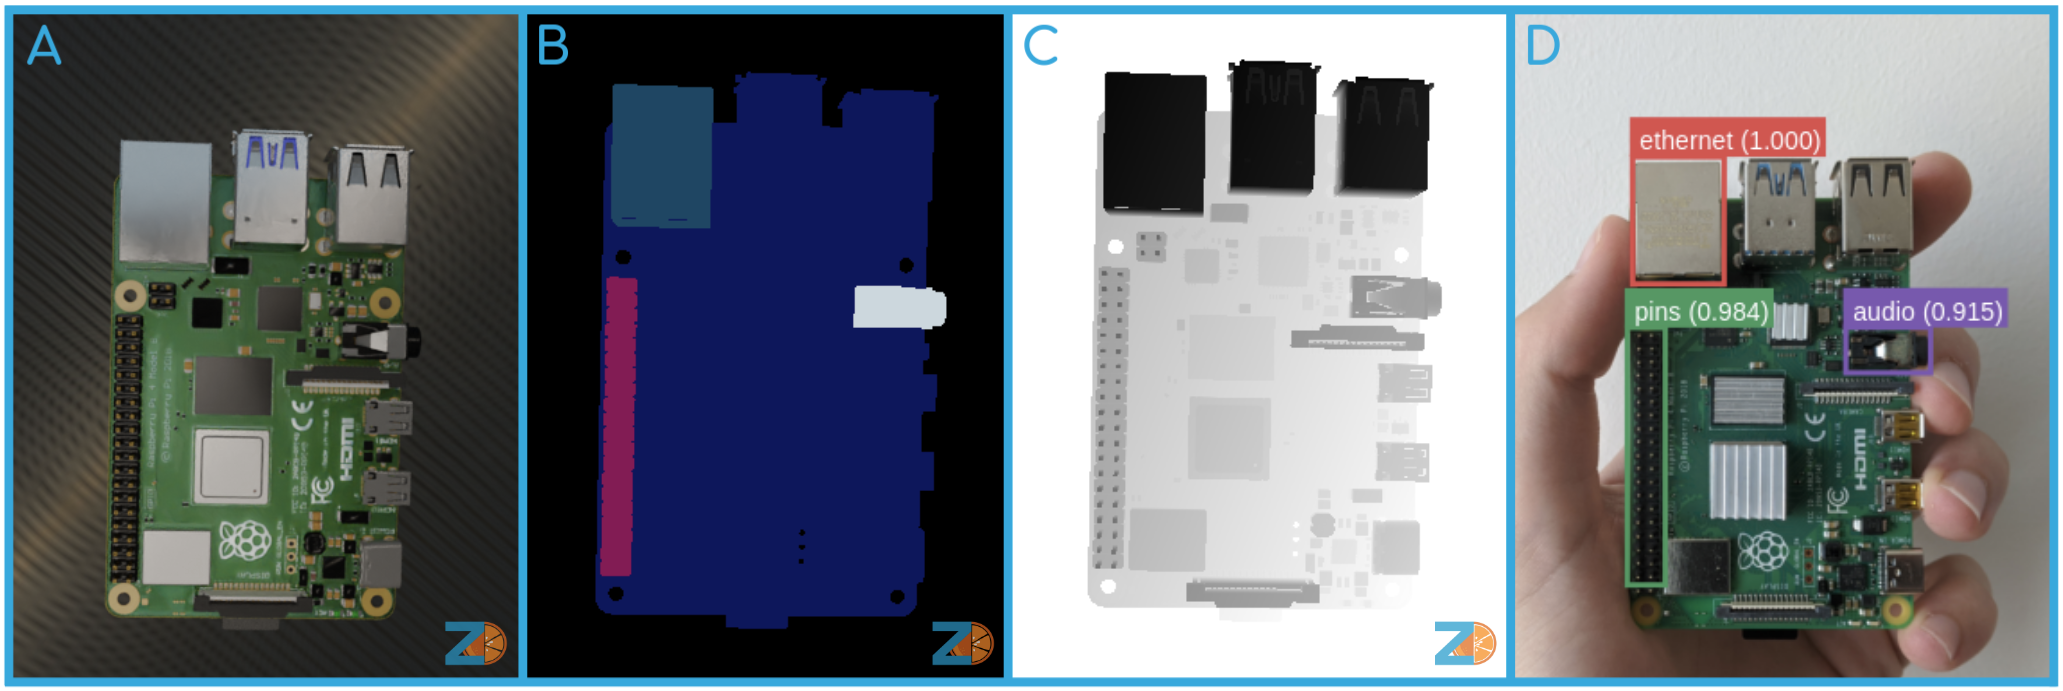
\includegraphics[width=\textwidth]{cover.png}
	\caption{Synthetic images of a raspberri pi created with zpy: (A) color image, (B) segmentation image, (C) depth image. These images are used to train a deep learning model, which predicts bounding boxes on key components as seen in the (D) prediction image}
	\label{fig:fig1}
\end{figure}

\section{Introduction}
\label{sec:introduction}

Open source machine learning frameworks (references)

Deep learning has exploded in popularity due to large open source frameworks such as tensorflow and pytorch

What is synthetic data.

Challenges with synthetic data

Sim2Real Gap and domain randomization

Black box nature of ML

For a thorough review of synthetic data literature, we recommend readers go through Nikolenko's 2019 summary paper \citep{nikolenko2019synthetic}.

\section{Background}
\label{sec:background}

\subsection{3D}
\label{sec:3d}

3D, short for the three dimensions of space we live in, is a catch-all term used to describe the varied technologies used to create virtual worlds. 3D’s technology stack can be roughly split into two broad categories: \emph{asset creation} and \emph{asset scripting}. Asset creation \ref{sec:assetcreation} is the process of creating assets: virtual objects, scenes, and materials. Asset scripting \ref{sec:assetscripting} is the process of manipulating those assets and their interactions over the fourth dimension of time. Decades of progress have resulted in sophisticated software tools that make 3D workflows more automated and straightforward, but a significant amount of human expertise and artistic talent is still required.

\subsubsection{Asset Creation}
\label{sec:assetcreation}

Assets are digital representations of a 3D object. One type of asset is a mesh: a connected graph of 3D points also called vertices, which define the surface of an object. Edges interconnect vertices, and a closed loop of vertices creates a polygon known as a face. The engineering and manufacturing world creates meshes using computer-aided design (CAD) software such as AutoCAD \citep{autocad}, Solidworks \citep{solidworks}, Onshape \citep{onshape}, and Rhino \citep{rhino}. The entertainment industry creates meshes using modeling software such as Maya \citep{maya}, 3DSMax \citep{3dsmax}, and Cinema4D \citep{cinema4d}.

Whereas a mesh describes the shape and form of an object, a material asset describes the texture and appearance of a virtual object. A material may define rules for the reflectivity, specularity, and metallic-ness of the object as a function of lighting conditions. Shader programs use materials to calculate the exact pixel values to render for each face of a mesh polygon. Modeling software usually comes packaged with tools for the creation and configuration of materials.

Finally, asset creation encompasses the process of scene composition. Assets can be organized into scenes, which may contain other unique virtual objects such as simulated lights and cameras. Deciding where to place assets, especially lights, is still almost entirely done by hand. Automatic scene composition remains a tremendous challenge in the 3D technology stack.

\subsubsection{Asset Scripting}
\label{sec:assetscripting}

The fourth perceivable dimension of our reality is time. Asset scripting is the process of defining the behaviors of assets within scenes over time. One type of asset scripting is called animation, which consists of creating sequential mesh deformations that create the illusion of natural movement. Animation is a tedious manual task because an artist must define every frame; expert animators spend decades honing their digital puppeteering skills. Specialized software is often used to automate this task as much as possible, and technologies such as Motion Capture (MoCap) can be used to record the movement of real objects and play those movements back on virtual assets.

Game Engines are software tools that allow for more structured and systematic asset scripting, mostly by providing software interfaces (e.g., code) to control the virtual world. Used extensively in the video game industry after which they were named, examples include Unity \citep{unity3d}, Unreal Engine \citep{unrealengine}, GoDot \citep{godot}, and Roblox \citep{roblox}. These game engines support rule-based spawning, animation, and complex interactions between assets in the virtual world. Programming within game engines is a separate skillset to modeling and animating and is usually done by separate engineers within an organization.

\subsubsection{Blender}
\label{sec:blender}

Blender is an open-source 3D software tool initially released in 1994 \citep{blender}. It has grown steadily over the decades and has become one of the most popular 3D tools available, with a massive online community of users. Blender’s strength is in its breadth: it provides simple tools for every part of the 3D workflow, rather than specializing in a narrow slice. Organizations such as game studios have traditionally preferred specialization, having separate engineers using separate tools (such as Maya for modeling and Unreal Engine for scripting). However, the convenience of using a single tool, and the myriad advantages of a single engineer being able to see a project start to finish, make a strong case for Blender as the ultimate winner in the 3D software tools race. 

Many of the world’s new 3D developers opt to get started and build their expertise in Blender for its open-source and community-emphasizing offering. This is an example of a common product flywheel: using a growing community of users to improve a product over time. With big industry support from Google, Amazon, and even Unreal, Blender also has the funding required to improve its tools with this user feedback.

In addition to supporting the full breadth of the 3D workflow, Blender has the unique strength of using Python as the programming language of choice for asset scripting. Python has emerged as the lingua franca for modern deep learning, in part due to the popularity of open-source frameworks such as TensorFlow \citep{tensorflow}, PyTorch \citep{pytorch}, and Scikit-Learn \citep{scikit-learn}. Successful adoption of synthetic data will require Machine Learning Engineers to perform asset scripting, and these engineers will be much more comfortable in Blender’s Python environment than Unity's C\# environment or Unreal Engine’s C++ tools.

\section{Motivation}
\label{sec:motivation}

\subsection{Democratization of Data}

The datasets used by companies today are almost exclusively collected. Images and annotations are gradually saved as they are generated by users of a product. Collecting a dataset large enough to train a robust machine learning model can take years.

Only companies that have the scale and have set up the infrastructure to collect and store large datasets will have the datasets required to train models.

In order to compete, small or newly formed companies often resort to purchasing data from a third party supplier. This market for the selling and reselling of collected data presents an existential threat to privacy. Though some regulations have emerged, famously GDPR in Europe, these have yet to change the landscape of the market for collected data.

The high cost of data labeling makes it unavailable to those without huge resources

\subsection{Fairness and Bias}

The real world is biased and unfair.

ML systems trained on this data will reflect the same bias during inference.

\begin{figure}
	\centering
	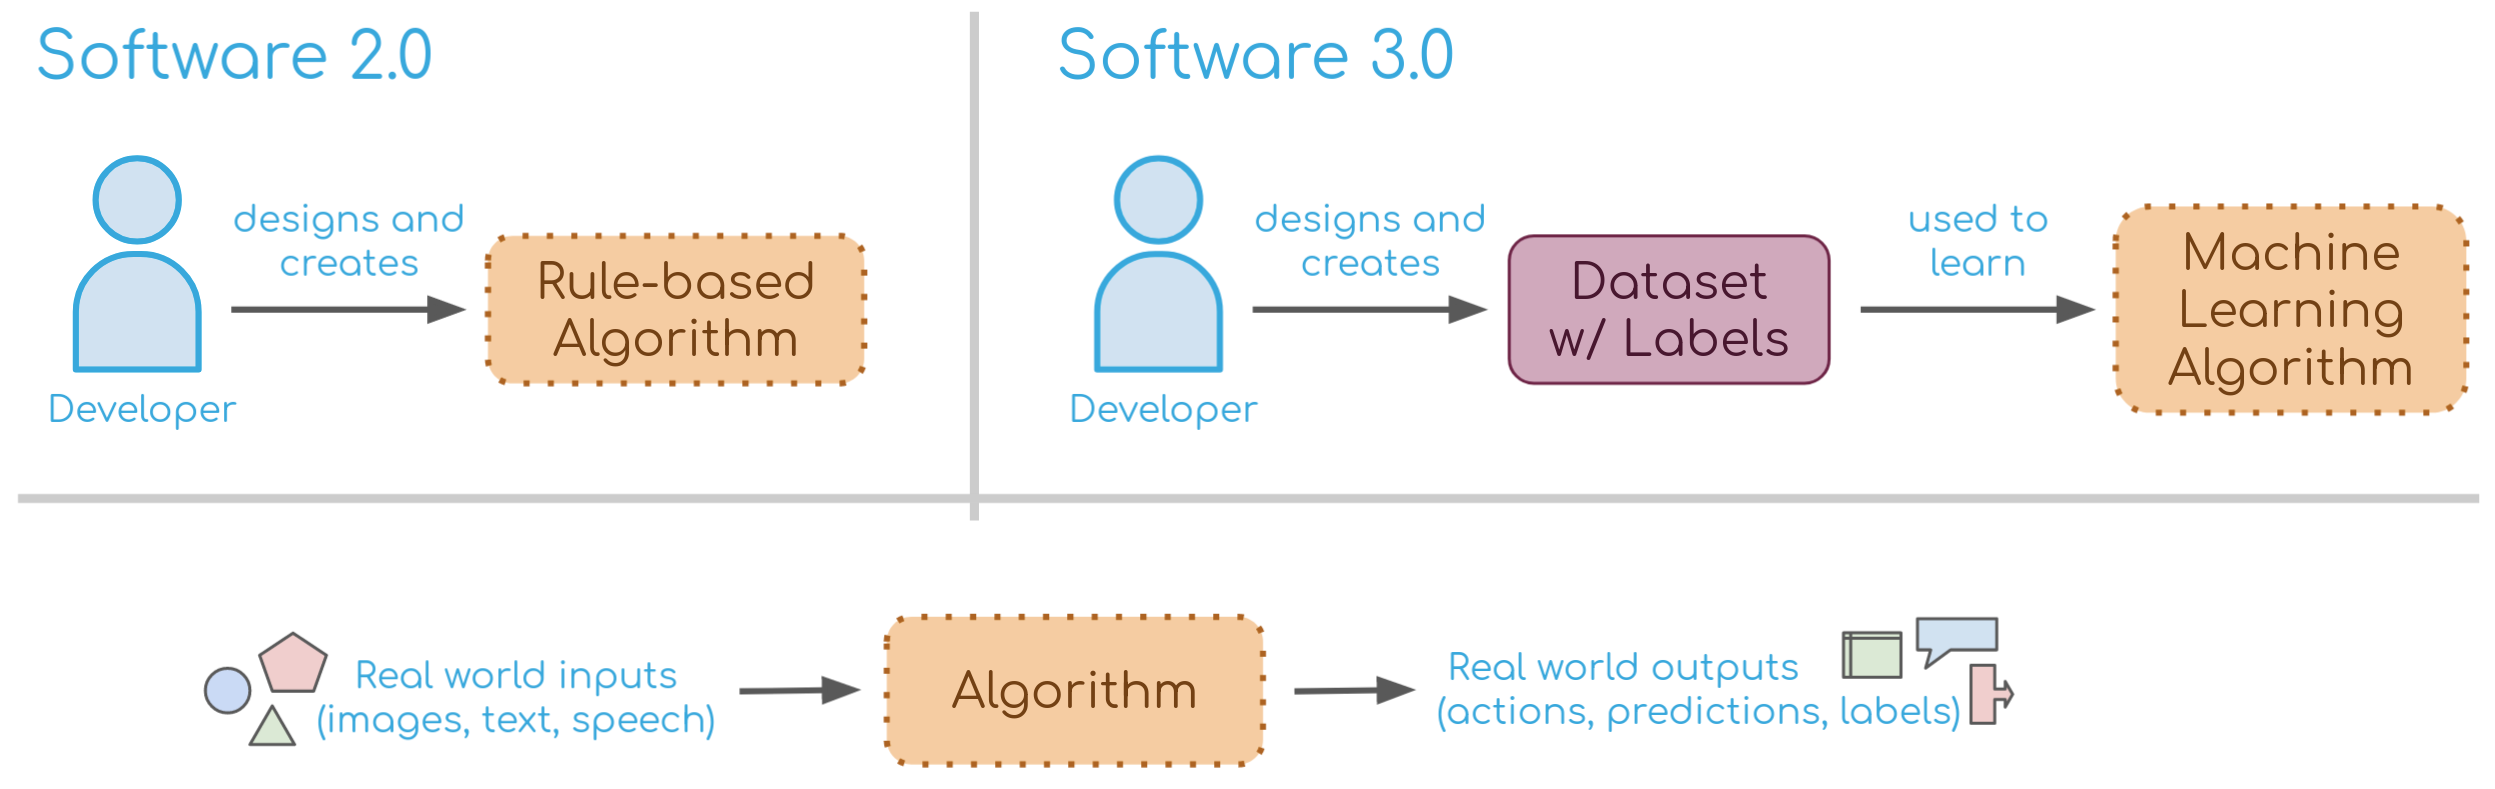
\includegraphics[width=\textwidth]{software3.png}
	\caption{Software 3.0: the developer transitions from writing explicit algorithms to creating and curating datasets which are used to train machine learning models.}
	\label{fig:fig2}
\end{figure}

\subsection{Software 3.0}
\label{sec:software3.0}

Data creation as a new paradigm for “programming”.

In the software world today, developers write explicit sets of rules (known as algorithms). These algorithms are then deployed into production systems, which consume input data and output actions.

In the software of tomorrow, developers will curate a dataset which will be used to train a deep learning model. This model will then be deployed into a production system, which will consume input data and output actions. This changes the workflow of developers from explicitly writing rules to instead creating the datasets which are then parsed to create algorithms.

\begin{figure}
	\centering
	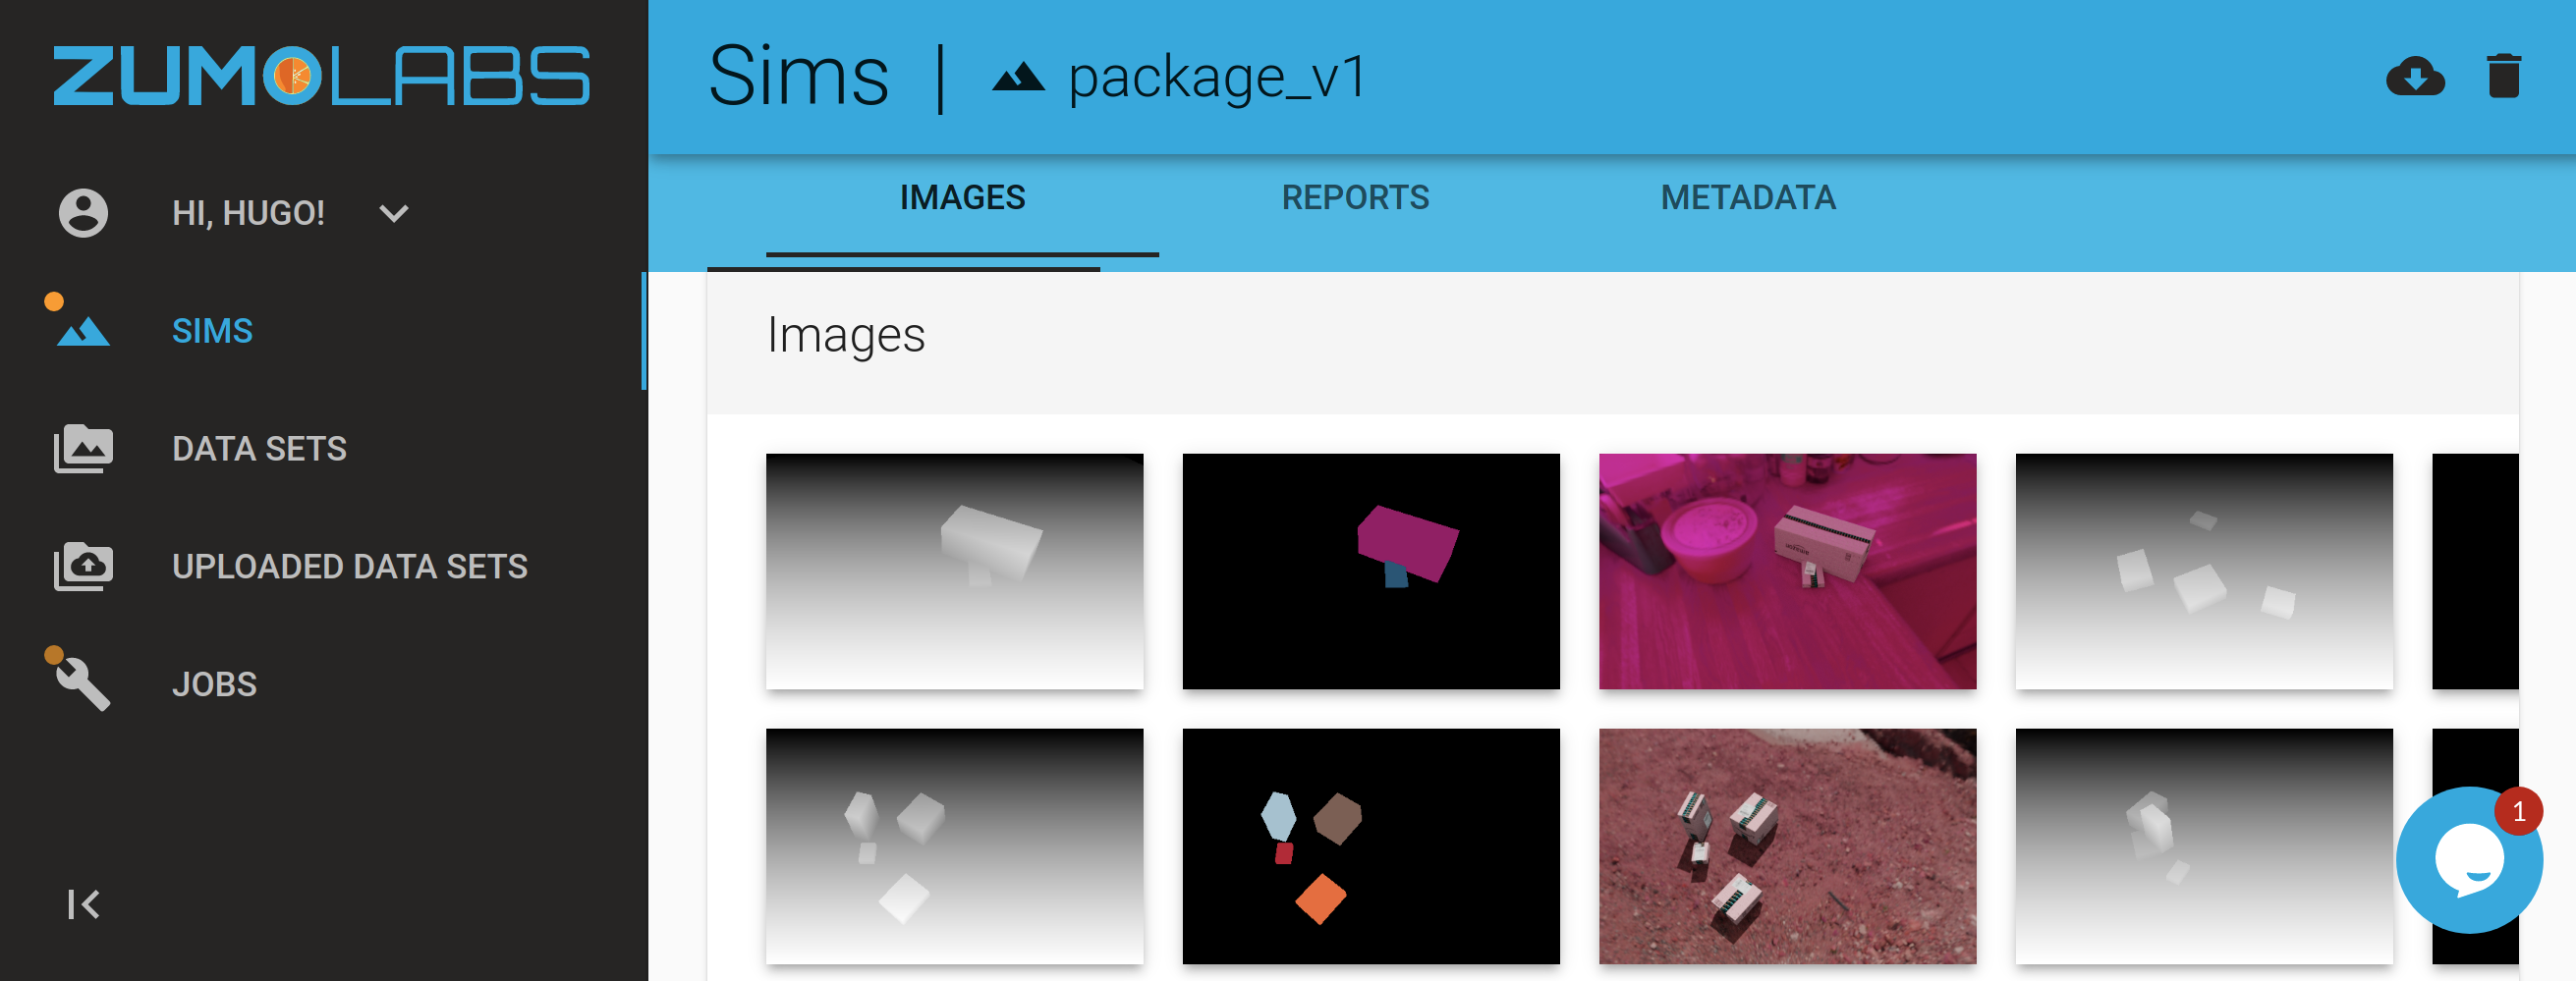
\includegraphics[width=\textwidth]{webapp.png}
	\caption{A visual interface for synthetic data creation via a WebApp.}
	\label{fig:webapp}
\end{figure}

\section{Project Features}
\label{sec:projectfeatures}

In this section we outline the key features and components of the zpy synthetic data toolkit.

\subsection{Blender Addon}
\label{sec:blenderaddon}

Blender allows for user-created AddOns, and provides tooling for integrating addon functionality with the Blender UI. Examples of popular AddOns are NodeWrangler and Botaniq. NodeWrangler adds simple productivity functionality to the Node System, a method of visual scripting common to 3D tools. Botaniq is a library of tree and plant assets, with a built in scattering method hugely popular due to the complexity of creating grass and trees from scratch. Blender users are comfortable installing and using addons as part of their workflow. The zpy-addon allows for mouse and button based versions of the segmentation, sim run script execution, and sim exporting workflows. Though these actions are possible entirely through python code, providing convenient button versions in a UI makes these processes available to a larger community of 3D artists who are not as comfortable in a code-only environment.

\subsection{Cloud Backend}
\label{sec:cloudbackend}

Computing has traditionally relied on Moore’s Law to increase the power of individual computers. In the past decade the individual compute power of a single computer has not increased significantly, and instead the ability to coordinate a large number of individual computers on a single task has become the method for increasing computation. This type of parallel computing has been democratized through the availability of cloud computing platforms such as AWS, GCP, and Azure. However, these platforms remain difficult for the average developer to use effectively, and domain experts are usually required to take software running on a single computer and scale it across many computers in parallel.

Abstracting away the difficulties of the cloud workflow and providing an intuitive and convenient interface for parallelizing computation is thus important for the synthetic data workflow. Dataset generation jobs can be made with the zpy CLI and API such that many computers are used, thus speeding up the generation job.

\subsection{User Interfaces}
\label{sec:userinterfaces}

We provide three different interfaces to interact with our product: a Python API \ref{lst:api}, a CLI \ref{lst:cli}, and a graphical WebApp \ref{fig:webapp}. Power users want an API (application programming interface) and CLI (command line interface). Building a ramp for the bulk of the developer community requires a GUI.

\begin{lstlisting}[language=Python,caption={Generating a dataset using the zpy python API.},label={lst:api}]
import zpy
zpy.generate()
\end{lstlisting}

\begin{lstlisting}[language=bash,caption={Generating a dataset using the zpy CLI},label={lst:cli}]
# First you will need to log in and set the project (image generation gets billed according to project)
zpy login $USERNAME 
zpy project set $PROJECT_UUID

# Generate the dataset
zpy create dataset "redbull cans and packs" can_v6 num_images 1000
\end{lstlisting}

\subsection{Python Module}
\label{sec:python module}

Hidden complexity

When designing software systems, there is usually a tradeoff between flexibility and simplicity. Simplicity is the ability to perform a task with minimal amount of work and a limited understanding of the software package. Flexibility is the ability to support many different tasks and allow for customization.

Random hdri and textures use default random textures unless a specific path is given

As explained in section X, deep learning is a python-first discipline. If we wish to include deep learning practitioners in the 3D stack it is thus of critical importance that we provide a python interface for the 3D workflow.

One of the core features of Python is the language’s human readable syntax. Python does not enforce function and variable type annotations, which makes it quicker to prototype code.

Functions in zpy are flexible in the arguments that they accept. The `zpy.opject.segment()` function call can accept an object directly of type `bpy.types.Object`, but it will also accept the unique string name of that object. 

Zpy modules are separated by dependencies

Zpy modules are independent of each other, a monolithic system is much harder to update and maintain

\begin{figure}
	\centering
	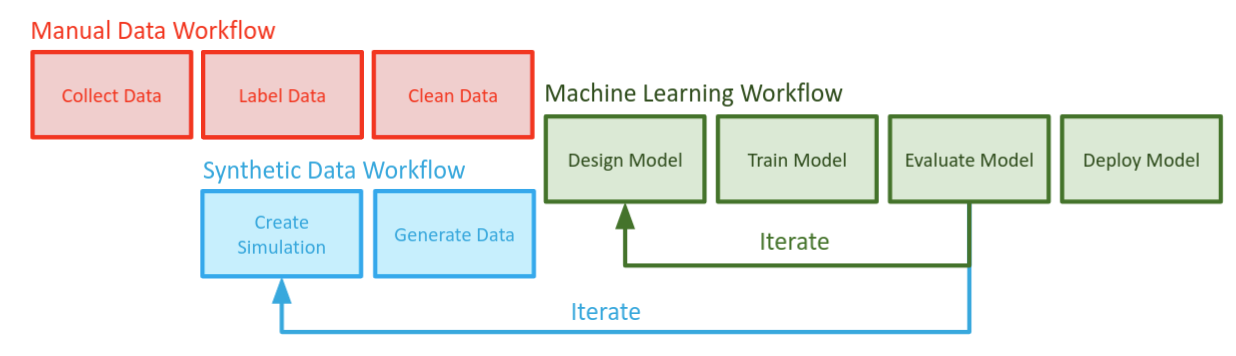
\includegraphics[width=\textwidth]{workflow.png}
	\caption{The synthetic data workflow allows for iteration of the dataset, unlike the manual data workflow, which depends on data collection.}
	\label{fig:workflow}
\end{figure}

\section{Workflow}
\label{sec:workflow}

The full workflow for synthetic data can be reduced into four key steps: \emph{Simulation Creation} \ref{sec:worflowsimcreation}, \emph{Dataset Generation} \ref{sec:generation}, \emph{Model Evaluation} \ref{sec:evaluation}, \emph{Iteration} \ref{sec:iteration}. The synthetic data workflow is similar to the workflow when using collected data, with the key exception that it allows for iteration on the dataset itself \ref{fig:workflow}.

\subsection{Simulation Creation}
\label{sec:worflowsimcreation}

The first step in the syntehtic data workflow is to design and create the \emph{sim}, short for simulation. A sim is a collection of 3D assets controlled at runtime through a single script called the \emph{run script}. The run script defines a function \lstinline{run(**kwargs)}, which acts as the point of entry for any generation process. Important parameters that configure the behavior of the run script are defined as kwargs, short for keyword arguments, in the \lstinline{run(**kwargs)} function. These kwargs allow configuration of the simulation through gin-config, a python package for configuration of python libraries \citep{ginconfig}.

The run script can be broken into two sections: the \emph{setup} and the \emph{loop}. The setup is executed first and typically only once. Setup can include code for creating categories, loading assets, and storing the pose of virtual objects in the scene. The loop, named after the \lstinline{for} loop python pattern, is repeated for some number of frames. Each frame can include code for jittering, saving annotations, and rendering images.

\begin{lstlisting}[language=Python,caption={Basic structure of the run function in a sim run script.},label={lst:setuploop}]
def run(**kwargs):
	# Setup Code
	for frame in zpy.blender.step():
		# Loop Code
\end{lstlisting}


\subsection{Dataset Generation}
\label{sec:generation}

Once a sim has been created it can be used to generate data. There is no constraint on the type of data a sim can generate, though images are the most common. Each frame of the loop in a run script will render out color and segmentation images. Datasets can be generated locally directly inside the Blender GUI through the zpy Blender AddOn \ref{sec:blenderaddon}. This makes sim development possible by making the local debuggin loop faster. Once a sim is properly generating data locally, it can be exported and uploaded to the cloud backend. Exporting is done through the Blender AddOn, and will create a zip file which contains all the asset dependencies required for sim execution. The exported sim can be uploaded to the cloud backend through any of the user interfaces described in \ref{sec:userinterfaces}.

Datasets can be generated in parallel, with multiple cloud machines running concurrent instances of the same sim. Each machine is given a different random seed, resulting in a unique dataset. The resulting collection of smaller datasets can be packaged into into a single larger dataset, making it easier for a machine learning practitioner to download and work with the dataset. Additional workflows are provided for sorting individual datapoints into test, train, and validation buckets.

\subsection{Model Evaluation}
\label{sec:evaluation}

Machine learning models are trained on a dataset for some time, and periodically evaluated on validation and test datasets. Model performance in computer vision can be measured in a variety of ways, such as precision and recall, or more aggregate metrics like mean average precision (mAP). Picking the right metric is problem specific and usually comes down to which type of failure is the most important: false positives or false negatives. It is important to note that though quantitative metrics are convenient, there is no replacement for qualitative analysis of model performance. We recommend that anyone building computer vision models take the time to examine model predictions on real images.

\subsection{Iteration}
\label{sec:iteration}

Those familiar with machine learning model development are aware of \emph{hyperparameters}: parameters whose value are used to control the learning process. Common examples of these include batch size, learning rate, and training epochs. These parameters, unlike the weights inside the model with are learned through training, must be set by the experiment designer. In practice, a human will use their intuition to decide upon a set or range of possible values for these hyperparameters, and then sweep over the possible hyperparameter space to find the best values for a given problem. This process, known as tuning, can have a high cost in engineering time and compute footprint. A technique known as AutoML has improved tuning by significantly reducing the engineering time cost. In AutoML, an automated process will tune these hyperparameters over time by trying different permutations, usually guided through a single heuristic score.

The kwargs of the run function in a sim are effectively additional hyperparameters that can also be tuned. The human designer of the sim can define plausible values and ranges for these sim hyperparameters, and then use an AutoML-like system to discover the values that result in the best model. This presents a unique opportunity in the machine learning workflow, where the dataset used to train a model is no longer static, and can be tuned and improved over time.

\section{Example}
\label{sec:example}

To put into practice what this paper has explained, we present an example of how synthetic data can be used to train a computer vision model. In this example, we train a detection model which is tasked with predicting the bounding boxes for packages and parcels in images. In section \ref{sec:domainrandomization} we explore the effect of some key dataset hyperparameters on the final model performance. In section \ref{sec:curicculum} we discuss how training curriculum can affect model performance when using synthetic data.

Following the synthetic data workflow,

Armed with our synthetic training dataset and our real test dataset, we are ready to do some model training.

We used a ResNet model implemented in PyTorch inside of the Detectron2 computer vision library \citep{wu2019detectron2}.


\subsection{Domain Randomization}
\label{sec:domainrandomization}

Domain randomization is a technique commonly used in synthetic data to increase the variance of a dataset distribution. In the field of synthetic data for computer vision, it might refer to randomizing the intensity of lighting in every frame of a simulation. Domain randomization is also important in the space of material assets: using a large variety of textures and material properties will help prevent texture overfitting, a common issue with CNNs \citep{DBLP:journals/corr/abs-1811-12231}. 

In our package experiment, we expose two boolean toggles as run function kwargs that are categorized as forms of domain randomization. One toggle enables domain randomization in the lighting space: changing the position and intensity of several lights in the sim. The second toggle enables random HDRIs, which change the appearance of the background in the package images.

\subsection{Training Curicculum}
\label{sec:curicculum}

Pre-training w/ real and fine-tuning on synthetic

Training only on synthetic

Training on mixed synthetic and real

\section{Conclusion}
\label{sec:conclusion}

TODO

\bibliographystyle{abbrvnat}
\bibliography{references}

\end{document}
